%!TEX program = xelatex
\documentclass[UTF8,zihao=-4]{ctexbook}
\usepackage{cite}
\usepackage{amsmath}
\usepackage{graphicx}
\usepackage{tikz}

\usepackage{stmaryrd}  % \talloblong

\graphicspath{{image/}}

%字体号设置
% \setCJKmainfont{SimSun}
% \setCJKmonofont{SimSun}
% \setmainfont{Times New Roman}
%%\normalsize{}

\setCJKmainfont{SimSun}
\setCJKmonofont{SimSun}
\setmainfont{Times New Roman}

\newcommand{\chuhao}{\fontsize{42pt}{\baselineskip}\selectfont}     %初号
\newcommand{\xiaochuhao}{\fontsize{36pt}{\baselineskip}\selectfont} %小初号
\newcommand{\yihao}{\fontsize{28pt}{\baselineskip}\selectfont}      %一号
\newcommand{\erhao}{\fontsize{21pt}{\baselineskip}\selectfont}      %二号
\newcommand{\xiaoerhao}{\fontsize{18pt}{\baselineskip}\selectfont}  %小二号
\newcommand{\sanhao}{\fontsize{15.75pt}{\baselineskip}\selectfont}  %三号
\newcommand{\sihao}{\fontsize{14pt}{\baselineskip}\selectfont}%     四号
\newcommand{\xiaosihao}{\fontsize{12pt}{\baselineskip}\selectfont}  %小四号
\newcommand{\wuhao}{\fontsize{10.5pt}{\baselineskip}\selectfont}    %五号
\newcommand{\xiaowuhao}{\fontsize{9pt}{\baselineskip}\selectfont}   %小五号
\newcommand{\liuhao}{\fontsize{7.875pt}{\baselineskip}\selectfont}  %六号
\newcommand{\qihao}{\fontsize{5.25pt}{\baselineskip}\selectfont}    %七号


\ctexset {
    chapter = {
        format = \linespread{1.0}\sanhao\bfseries\heiti\centering,
        nameformat = {},
        titleformat = {},
        number = \arabic{chapter},
        numberformat = \rmfamily,
        aftername = \quad,
        beforeskip = {7pt},
        afterskip = {18pt},
        pagestyle = plain,
    }
}
%- section
\ctexset {
    section = {
        format = \linespread{1.0}\sihao\bfseries\CJKfamily{song}\centering,
        numberformat = \rmfamily,
        aftername = \quad,
        beforeskip = {24pt},
        afterskip = {6pt},
    }
}
%- subsection
\ctexset {
    subsection = {
        format = \linespread{1.0}\zihao{-4}\bfseries\CJKfamily{song}\raggedright,
        numberformat = \rmfamily,
        aftername = \quad,
        beforeskip = {12pt},
        afterskip = {6pt},
    }
}
%- subsubsection
\ctexset {
    subsubsection = {
        format = \linespread{1.0}\zihao{-4}\CJKfamily{song}\raggedright,
        numberformat = \rmfamily,
        aftername = \quad,
        beforeskip = {12pt},
        afterskip = {6pt},
    }
}

%% 页面设置
\usepackage{geometry}
\geometry{papersize={21.0cm,29.7cm}}
\geometry{left=3.18cm,right=3.18cm,top=2.54cm,bottom=2.54cm}

\title{有限自动机最小化算法的分类}
\author{胡双朴}
\date{2019.03}

\tolerance=1
\emergencystretch=\maxdimen
\hyphenpenalty=10000
\hbadness=10000

%% 下划线
\usepackage{ulem}

\usepackage{fancyhdr}
\pagestyle{fancy}
% \lhead{ }
% \chead{ }
% \rhead{ }
% \lfoot{}
\cfoot{\thepage}
\rfoot{}
\renewcommand{\headrulewidth}{0.4pt}
\renewcommand{\headwidth}{\textwidth}
\renewcommand{\footrulewidth}{0pt}

\usepackage[colorlinks,linkcolor=black,anchorcolor=blue,citecolor=red]{hyperref}

\usepackage{listings}
\usepackage{xhfill}
\usepackage{color}
\definecolor{codegreen}{rgb}{0,0.6,0}
\definecolor{codegray}{rgb}{0.5,0.5,0.5}
\definecolor{codepurple}{rgb}{0.58,0,0.82}
\definecolor{backcolour}{rgb}{0.99,0.99,1.0}
 
\lstdefinestyle{mystyle}{
    backgroundcolor=\color{white},   
    commentstyle=\color{codegreen},
    keywordstyle=\color{magenta},
    numberstyle=\tiny\color{codegray},
    stringstyle=\color{codepurple},
    basicstyle=\footnotesize\ttfamily,
    breakatwhitespace=false,         
    breaklines=true,                 
    captionpos=b,                    
    keepspaces=true,                 
    numbers=left,                    
    numbersep=5pt,                  
    showspaces=false,                
    showstringspaces=false,
    showtabs=false,                  
    tabsize=2
}


\begin{document}



%%目录页
%\newpage
% \section*{目录}
\addcontentsline{toc}{section}{目录}
\tableofcontents

\thispagestyle{empty}


%%正文页
\newpage
\setcounter{page}{1}

\section{介绍}

自1950年来,确定性有限自动机的最小化就一直在研究当中。简单来说就是找到一个唯一的(直至同构)最小的确定性有限自动机,它能接收与给定的确定性有限自动机相同的语言。解决这一问题的算法应用范围很广,从编译器构造到硬件电路的最小化都有它的身影。有了形式多样的应用程序,不同的表示形式的数量也在增加:大多数教科书都有自己的变体,而时间复杂度最优的算法 (Hopcroft的算法) 仍然晦涩难懂。

本文介绍了有限自动机最小化算法的有关分类。如下所示:

\begin{itemize}
    \item[·] 大多数教材的作者称他们的最小化算法由 Huffman 算法 \cite{Huff54} 和 Moore 算法 \cite{Moor56} 直接推导得到。不幸的是,大多数教材都展示了截然不同的算法 (比如 \cite{AU92,ASU86,Hu79,Wood87}), 只有由 Aho 和 Ullman 发表的算法直接源自 \cite{Huff54, Moor56}。
    \item[·] 虽然大多数算法依赖于计算状态的等价关系,但伴随算法演示的许多解释并未明确提及算法是计算等价关系、它包含的状态划分还是它的补充。
    \item[·] \uline {Comparison of the algorithms is further hindered by the vastly differing styles of presentation --- sometimes as imperative programs or as functional programs, but frequently only as a descriptive paragraph. 算法之间的比较进一步受到呈现方式的巨大差异的阻碍。有时作为命令式程序或函数式程序,但通常只作为描述性段落。}
\end{itemize}
A related taxonomy of finite automata construction algorithms appears in [Wats93].\\
有限自动机构造算法的相关分类在\cite{Wats93}中。

\uline{All except one of the algorithms rely on determining the set of automaton states which are equivalent.} The algorithm that does not make use of equivalent states is discussed in Section 2. In Section 3 the definition and some properties of equivalence of states is given. Algorithms that compute equivalent states are presented in Section 4. The main results of the taxonomy are summarized in the conclusions Section 5. Appendices A and B give the basic definitions required for reading this paper. The definitions related to finite automata are taken from [Wats93]. The minimization algorithm relationships are shown in a "family" tree\ in Figure 1.

\uline{除了一个算法之外,其他所有算法依赖于确定的等价}\footnote{状态的等价稍后定义。}\uline{的自动机状态的集合。}在第2节中讨论了不使用等价状态的算法。在第3节中给出了状态等价的定义和一些性质。计算等效状态的算法在第4节中给出。分类的主要结果被总结在结论部分5中。附录A和附录B给出了阅读本文所需的基本定义。与有限自动机相关的定义取自\cite{Wats93}。图1中的“Family tree”中显示了最小化算法之间的关系。

The principal computation in most minimization algorithms is the determination of equivalent (or inequivalent) states —— thus yielding an equivalence relation on states. In this paper,we consider the following minimization algorithms:

大多数最小化算法的主要计算是确定等价的(或不等价的)状态,从而在状态上产生等价关系。在本文中,我们考虑以下最小化算法:

\begin{itemize}
    \item[·] Brzozowski's (possibly nondeterministic) finite automaton minimization algorithm as presented in [Brzo62]. This elegant algorithm (Section 2) was originally invented by Brzozowski, and has since been re-invented without credit to Brzozowski. Given a (possibly nondeterministic ) finite automaton without E-transitions, this algorithm produces the minimal deterministic finite automaton accepting the same language.
    
    Brzozowski(可能是非确定性的)有限自动机最小化算法 在 \cite{Brzo62} 中提出。这个优雅的算法(第2节)最初是由Brzozowski提出,此后又在没有Brzozowski的“参与”的情况下被重新提出。在没有 $\epsilon$-跃迁的情况下,给出了一个(可能不确定的)有限自动机,\uline{该算法产生最小的确定性有限自动机接受相同的语言}。

    \item[·] Layerwise computation of equivalence as presented in [Wood87, \cite{Moor56} Brau88, Urba89]. This algorithm (Algorithm 4. 2) is a straightforward implementation suggested by the approximation sequence arising from the fixed-point definition of equivalence of states. 

    分层等价计算等价于 \cite{Wood87, Moor56, Brau88, Urba89} 中提出。算法(算法 4.2)是由状态等价的定点定义产生的近似序列所建议的直接实现。

    \item[·] Unordered computation of equivalence This algorithm (Algorithm 4.3, not appearing in the literature) computes the equivalence relation; pairs of states (for consideration of equivalence) are chosen in an arbitrary order.

    等价无序计算。该算法(算法4.3,未出现在文献中)计算等价关系;以任意顺序选择状态对(考虑等价性)。

    \item[·] Unordered computation of equivalence classes as presented in [ASU86]. This algorithm (Algorithm 4.4)is a modification of the above algorithm computing equivalence of states.

    等价类的无序计算发表在\cite{ASU86}。该算法(算法4.4)是上述算法计算状态等价性的一种更改。

\end{itemize}

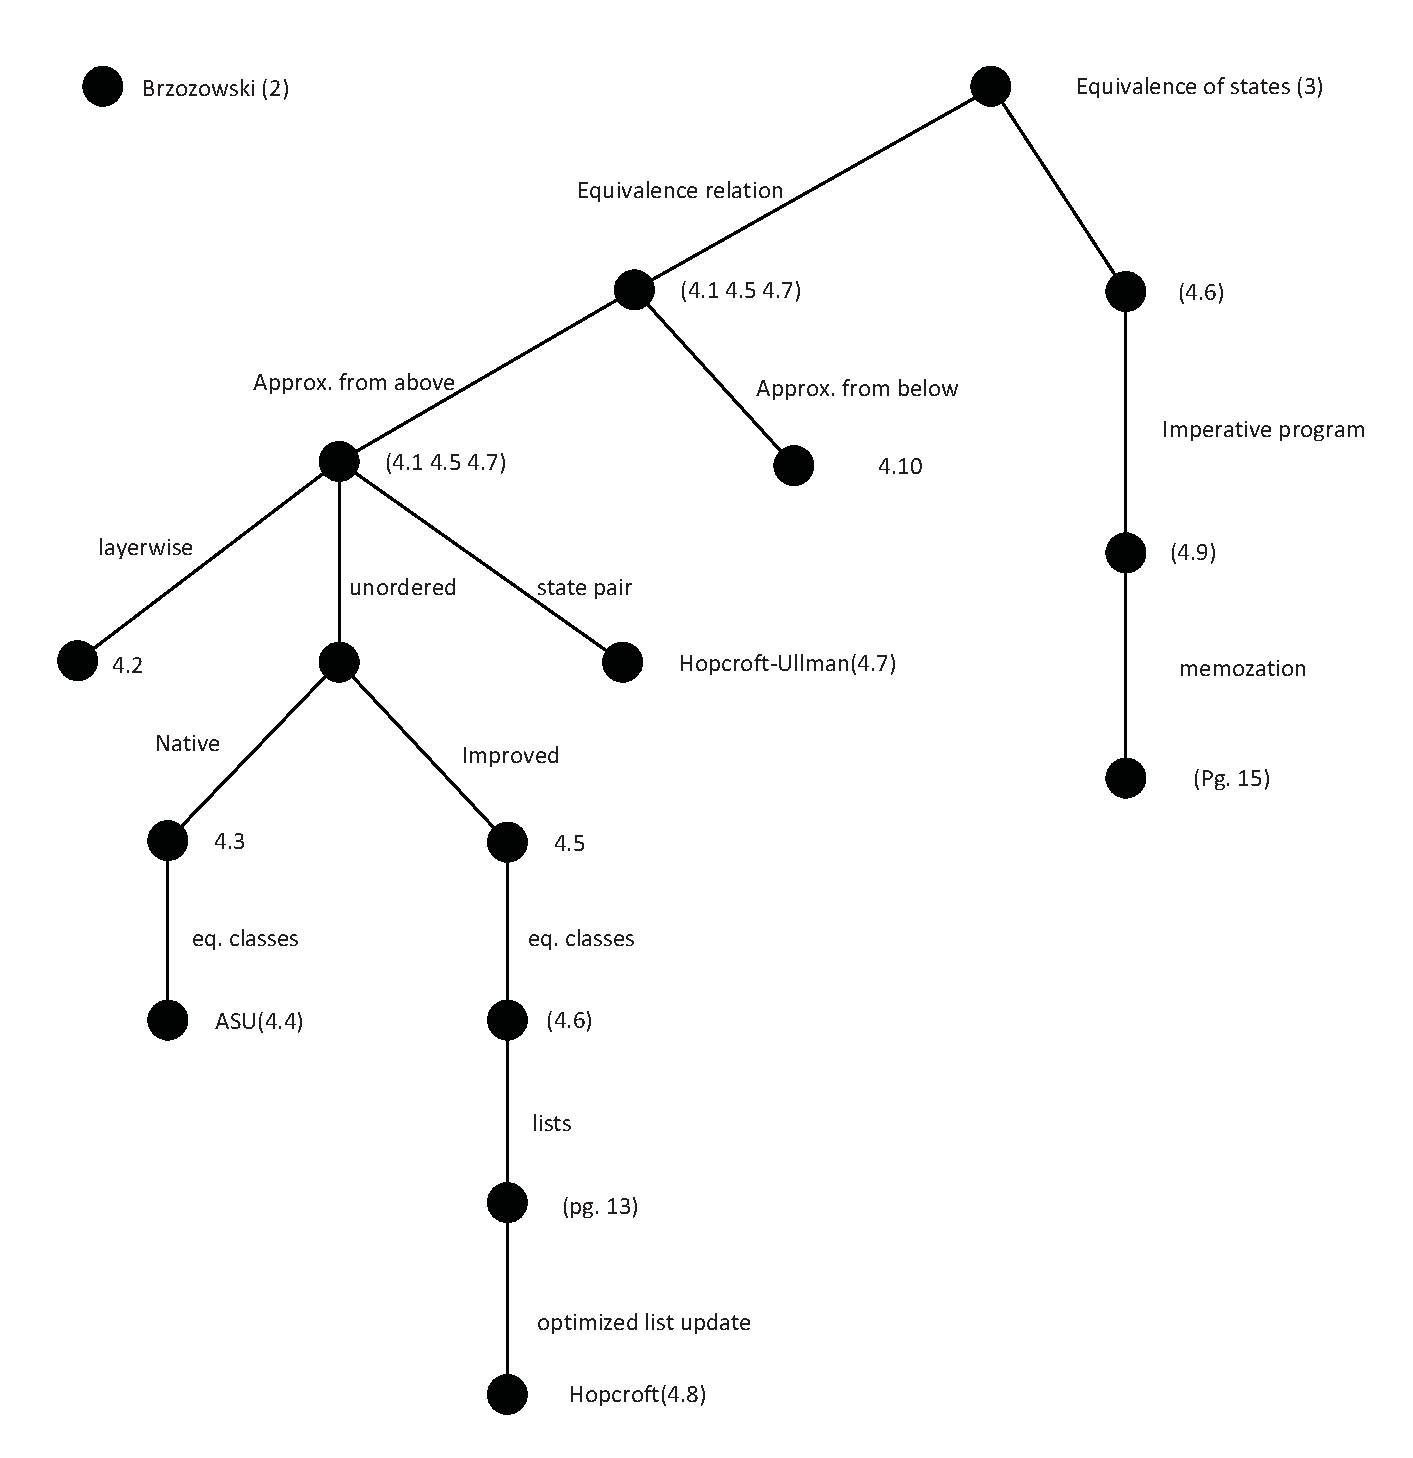
\includegraphics[width =.9\textwidth]{Family_tree.eps}

Figure 1: The family trees of finite automata minimization algorithms. Brzozowski's minimization algorithm is unrelated to the others, and appears as a separate(single vertex)tree. Each algorithm presented in this paper appears as a vertex in this tree. For each algorithm that appears explicitly in this paper, the construction number appears in parentheses(indicating where it appears in this paper). For algorithms that do not appear explicitly, a reference to the section or page number is given. Edges denote a refinement of the solution (and therefore explicit relationships between algorithms). They are labeled with the name of the refinement.

图1:有限自动机最小化算法的“Family tree”。Brzozowski的最小化算法与其他算法无关,并作为一个单独的(单顶点)树出现。本文提出的每一个算法都作为树的顶点出现。对于本文中明确出现的每个算法,构造数在括号中(标示它在本文中出现的位置)。对于未显式显示的算法,给出了相应的页码。边表示解的\uline{细化}(也即算法之间的显式关系)。它们被标记为\uline{细化}的名称。

\begin{itemize}

    \item[·] Improved unordered computation of equivalence. This algorithm (Algorithm 4.5, not appearing in the literature) also computes the equivalence relation in all arbitrary order. The algorithm is a minor improvement over the other unordered algorithm.
 
    改进的等价的无序计算。这个算法(算法4.5,没有出现在文献中)也以任意顺序计算等价关系。该算法是对其他无序算法的一个小改进。

    \item[·] Improved unordered computation of classes. This algorithm (Algorithin 4.6, not appearing in the literature) is a modification of the above algorithm to compute the equivalence classes of states. This algoritm is used in the derivation of Hopcroft's minimization algorithin.
 
     改进了类的无序计算。该算法(算法4.6,不在文献中)是上述算法的修改,用来计算等价类的状态。该算法用于Hopcroft最小化算法的推导。

    \item[·] Hopcroft and Ullman's algorithm as presented in [HU79]. This algorithm (Algorithm 4.7) computes the inequivalence (distinguishability) relation. Although it is based upon the algorithus of Huffinan and Moore [Huff54, Moor 56], this algorithm uses some interesting encoding techniques.
 
    Hopcroft 和 Ullman 算法在\cite{Hu79}中提出。该算法(算法4.7)计算不等价(区分性)关系。虽然它是基于 Huffinan \cite{Huff54}和 Moore \cite{Moor56} 的算法,但该算法使用一些有趣的编码技术。

    \item[·] Hopcroft's algorithm as presented in [Hopc71, Grie73]. This algorithm (Algorithm 4.8)is the best known algorithm (in terms of running time analysis) for minimization. As the original presentation by Hopcroft is diflicult to understand, the presentation in this paper is based upon the one giveu by Gries.
 
    HopRofft的算法在 \cite{Hopc71, Grie73} 提出 。该算法(算法4.8)是用于最小化的最有名的算法(在运行时间分析方面)。由于 Hopcroft 的原始陈述是难以理解的,本文的介绍基于Gries的文章。

    \item[·] Pointwise computation of equivalence. This algorithm (Algorithm 4.9 not appearing in the literature) computes the equivalence of a given pair of states. It draws upon some nonautomata related techniques, such as: structural equivalence of types and memoization of functional programs.
 
    等价的点态计算。该算法(算法4.9,不在文献中)计算给定状态对的等价性。它借鉴了一些非自动机相关的技术,例如:类型的结构等价和函数式程序的记忆化。

    \item[·] \uline{Computation of equivalence from below (with respect to refinement). This algorithm (Algorithm 4.10, not appearing in the literature) computes the equivalence relation from below. } Unlike any of the other known algorithms, the intermediate result of this algorithm can be used to construct a smaller (although not minimal) deterministic finite automaton.
  \newline
    \uline{由下面的内容(关于细化)计算等价性。该算法(算法4.10,不在文献中)计算从下面的等价关系。}与任何其他已知算法不同,该算法的中间结果可用于构造较小的(虽然不是最小的)确定性有限自动机。

\end{itemize}
\chapter{Brzozowski提出的算法}

大多数最小化算法应用于 $DFA$ 。对于不确定的 $FA$,应该先应用子集构造,然后应用最小化算法。在本节中,我们将考虑在(未知的)算法之后应用子集构造(带无用状态删除)以生成最小$DFA$的可能性。我们现在构造这样的算法。(在本节中描述的算法也可用于通过用 $subset$ 替换函数 $subsetopt$ 来构造最小完全$DFA$)。

令$M_0 = (Q_0,V,T_0,\emptyset ,S_0,F_0)$ 为一个 $\epsilon$-$free$ $FA$,对其进行最小化,令 $M_2 = ( Q_2,V,T_2,\emptyset,S_2,F_2 ) $ 为最小的 $DFA$,那么 $ \mathcal{L} (M_0) = \mathcal{L}(M_2) $ ( $Min(M_2)$ 当然也是,详见定义 B.19)。(对本节中剩下的部分我们使用 $Minimal$(性质 B.21))。由于最后构造子集,有一些中间$FA$ $M_1 = ( Q_1,V,T_1,\emptyset,S_1,F_1 )$,于是$M_2 = useful \circ subsetopt(M_1)$。我们要求 $M_1$ 是由 $M_0$ 得到的,那么 $ \mathcal{L}_{FA}(M_2) = \mathcal{L}_{FA}(M_1) = \mathcal{L}_{FA}(M_0)$。

从 $Minimal(M_2)$  (性质 B.21)开始,我们需要:
$$ (\forall p,q,:p\in Q_2 \land q \in Q_2 \land p \not= q : \overrightarrow{\mathcal{L}}(p) \not= \overrightarrow{\mathcal{L}}(q)) \land useful(M_2)   $$ 
对与所有的状态$q\in Q_2$,由于 $M_2 = useful_s \circ subsetopt(M_1)$ ,所以有 $q\in P(Q_1$ 。性质 B.25 的子集构造给出: 
$$ (\forall p:p\in Q_2 : \overrightarrow{\mathcal{L}}(p) = (\cup q:q \in Q_1 \land q \in p:\overrightarrow{\mathcal{L}}(q)) ) $$ 
我们需要 $M_1$ 上充足的条件来确保 $Minimal(M_2)$。相应条件的推导如下: \\
\mbox{   } $Minimal(M_2)$ \\
\mbox{ } $\equiv$ \mbox{  } {$Minimal$的定义(性质 B.21)} \\
\mbox{   } $ (\forall p,q,:p\in Q_2 \land q \in Q_2 \land p \not= q : \overrightarrow{\mathcal{L}}(p) \not= \overrightarrow{\mathcal{L}}(q)) \land useful(M_2)$ \\
\mbox{ } $ \Leftarrow $ \mbox{  } { 性质 B.25; $M_2 = useful \circ subsetopt(M_1)$ } \\
\mbox{   }$ (\forall p,q,:p\in Q_2 \land q \in Q_2 \land p \not= q : \overrightarrow{\mathcal{L}}(p) \not= \overrightarrow{\mathcal{L}}(q) = \emptyset) \land useful(M_2)$ \\
\mbox{ } $\equiv $ \mbox{  } {$Det'$的定义(性质 B.18)和 $useful_s, Useful_f $(备注 B.13) } \\
\mbox{   } $Det'(M^R_1) \land Useful(M^R_1)$ \\
\mbox{ } $\Leftarrow $ \mbox{  } {$Det'(M) \Leftarrow Det(M)$} \\
\mbox{   } $Det(M^R_1) \land Useful(M^R_1)$ \\
$M_1$需要的条件可以通过 $M_1=R \circ useful_s \circ subsetopt \circ R(M_0)$ (反转前缀)建立。

完全最小化算法(对于任何 $\epsilon$-$free$ $M_0\in FA$ )如下:
$$  M_2 = useful_s \circ subsetopt \circ R \circ useful_s \circ subsetopt \circ R(M_0) $$

该算法最初由 Brzozowski 在 \cite{Brzo62} 中提出。最初 Jan van de Snepscheut 在他的博士论文 \cite{vdSn85}中提出该算法时,对该算法的描述是模糊的。在该论文中,算法来源于一个教授的私人通讯——埃因霍芬理工大学的 Pereman, Pereman 最初在 Mirkin 的文章 \cite{Mirk65} 中找到该算法。虽然 Mirkin 引用了 Brzozowski \cite{Brzo64} 的论文,但 Mirkin 的作品是否受 Brzozowki 的最小化工作的影响尚不清楚。Jan van de Snepscheut 的新书\cite{VDSn93} 描述了该算法,但既不提供该算法历史,也不提供该算法的引文(除了他自己的论文外)。


\chapter{状态等价最小化}
% 本节中,我们限定在完全的 DFA 的最小化中。\uline{This is strictly a notational convenience, as the minimization algorithm can be modified to work for non-complete DFA.严格地说,这是一种标记的便利,因为可以对最小化算法进行修改,使其适用于不完全DFA。} 除非$DFA$的语言是$V^*$,否则完全最小化$DFA$比不完全最小化DFA多一个状态(sink)。令 $ M = (Q,V,T,\emptyset,S,F)$ 为完全$DFA$,这个特殊的$DFA$将会贯穿本节内容。我们也假设所有的 $M$ 的所有状态都是开始状态可达的,也就是$Useful_s(M)$。由于 $M$ 是确定且完全的,我们也把转移关系 $T \in Q \times V \to Q$ 称为全函数,而不是 $T \in Q \times V \to \mathcal{P}(Q)$。
节中,我们限定在完全的 DFA 的最小化中。严格地说,这是一种书写方式上的便利,可以对最小化算法进行修改,使其适用于不完全DFA。 除非$DFA$的语言是$V^*$,否则完全最小化$DFA$比不完全最小化DFA多一个状态(sink)。令 $ M = (Q,V,T,\emptyset,S,F)$ 为完全$DFA$,这个特殊的$DFA$将会贯穿本节内容。我们也假设所有的 $M$ 的所有状态都是开始状态可达的,也就是$Useful_s(M)$。由于 $M$ 是确定且完全的,我们也把转移关系 $T \in Q \times V \to Q$ 称为全函数,而不是 $T \in Q \times V \to \mathcal{P}(Q)$。

为了最小化 $DFA$ $M$,我们计算等价关系 $E \subseteq Q \times Q$,将其定义为\\
$\mbox{   } (p,q) \in E \equiv ( \overrightarrow{\mathcal{L}}(p) = \overrightarrow{\mathcal{L}}(q) )$ \\
% \uline{Since this is an equivalence relation, we are really interested in unordered pairs of states. 由于这是一个等价关系,我们确实对无序状态对有兴趣},使用有序状态对比使用无序状态对更方便。
由于这是一个等价关系,我们对无序状态对有兴趣。使用有序状态对比使用无序状态对更方便。

根据等价关系 $E$ ,使用 \textit{merge} 转换来对等价关系进行合并。
\newline

\begin{transformation}[合并状态]
    对于任何满足 $ H \in E $ 的等价关系 $H$, 函数 $merge$ 可以用来减少 ${DFA}$的状态数\footnote{当$H$是状态上的恒等关系时,函数$merge$不会减少状态的数量。} ,函数 $merge$ 定义为:
    \begin{table}[!htbp]
        \centering
        %\small% fontsize
        \setlength{\tabcolsep}{4pt}% column separation
        \renewcommand{\arraystretch}{1.4}%row space 
        \begin{tabular}{lcll} 
            $merge((Q,V,T,\emptyset,\{s\},F),H)$ & = & {\bfseries let} & $T' = \{([p]_H,a,[q]_H):(p,a,q)\in T\}$ \\
                                                 &   & {\bfseries in}  &                                         \\
                                                 &   &                 & $ ([Q]_H,V,T',\emptyset,\{[s]_H\},[F]_H) $  \\
                                                 &   & {\bfseries end} &                               \\
        \end{tabular}
    \end{table}
\end{transformation}




% \begin{displaymath}
%     \begin{split}
%     & merge((Q,V,T,\emptyset,\{s\},F),H)  = \mbox{\textbf{let} }  T' = \{([p]_H,a,[q]_H):(p,a,q)\in T\} \\
%     & \mbox{              \textbf{in}}\\
%     & \mbox{                 } ([Q]_H,V,T',\emptyset,\{[s]_H\},[F]_H) \\
%     & \mbox{              \textbf{end}}
%     \end{split}
% \end{displaymath}

% 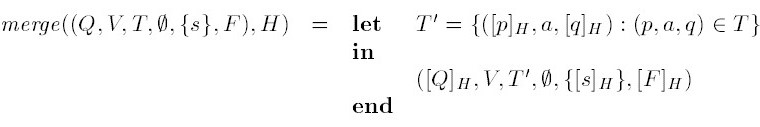
\includegraphics[width =.9\textwidth]{figure2.jpg}

$merge$ 的定义独立于等价类的代表的选择。函数 $merge$ 拥有以下性质:
\begin{equation*}
    \mathcal{L}_{FA}(merge(M,H)) = \mathcal{L}_{FA}(M) \land | merge(M,H) | \leq |M| \land | merge(M,H)| = \sharp H
\end{equation*}
它保留了 $Complete$, $\epsilon$-$free$, $Useful$, $Det$, 和 $minimal$ 等性质; 当然, $merge$ 仅定义在 $\epsilon$-$free$ 和 $DFA$ 上。

为了计算关系$E$, 需要函数$\overrightarrow{\mathcal{L}}$的一个性质。

\begin{property}[函数$\overrightarrow{\mathcal{L}}$]
    函数$\overrightarrow{\mathcal{L}}$ 满足
    \[ \overrightarrow{\mathcal{L}}(p) = (\cup a:a \in V : \{a\} \cdot \overrightarrow{\mathcal{L}}(T(p,a))) \cup ( \mbox{ \textbf{if} }   (p \in E) \mbox{ \textbf{then} }   \{\epsilon\} \mbox{ \textbf{else} }   {\emptyset  \mbox{ \textbf{fi} }}) \]
    这允许我们给出状态等价的另一种描述。
\end{property}

% \noindent{\textbf{性质3.2 (函数$\overrightarrow{\mathcal{L}}$)}: 函数$\overrightarrow{\mathcal{L}}$ 满足 }
% $$ \overrightarrow{\mathcal{L}}(p) = (\cup a:a \in V : \{a\} \cdot \overrightarrow{\mathcal{L}}(T(p,a))) \cup ( \mbox{ \textbf{if} }   (p \in E) \mbox{ \textbf{then} }   \{\epsilon\} \mbox{ \textbf{else} }   {\emptyset  \mbox{ \textbf{fi} }}) $$
% \uline{This allow us to give an alternate characterization of equivalence of states. 这允许我们给出状态等价的另一种描述}。  
% \newline

\begin{definition}[状态的等价]\label{def:eqstate}
    % \uline{等价关系 $E$ 是最大不动点}(在细化的情况下):
    等价关系 $E$ 是最大细化条件下的划分关系:
    \[ (p,q) = E \equiv ( p \in F \equiv q \in F ) \land ( \forall a:a \in V : (T(p,a),T(q,a)) \in E ) \]
    
\end{definition}

% \noindent{\textbf{定义 3.3 (状态的等价):} \uline{等价关系 $E$ 是最大不动点}(在细化的情况下): } \\
% $\mbox{  } (p,q) = E \equiv ( p \in F \equiv q \in F ) \land ( \forall a:a \in V : (T(p,a),T(q,a)) \in E )$
% \newline
% \\

\begin{remark}
    % \uline{the greatest fixed point has the least number of equivalence classes of any such fixed point. 最大不动点拥有最少的任何此类不动点的等价类数。}
    最大划分关系拥有最多的等价类数目。
\end{remark}

% \noindent{\textbf{备注3.4:} \uline{the greatest fixed point has the least number of equivalence classes of any such fixed point. 最大不动点拥有最少的任何此类不动点的等价类数。} }
% \newline

\begin{remark}
    定义 \ref{def:eqstate} 中的任何不动点都可以使用。为了最小化自动机,需要最大不动点。
\end{remark}

% \noindent{\textbf{备注3.5:} 定义 \ref{def:eqstate} 中的任何不动点都可以使用。为了最小化自动机,需要最大不动点。}
% \newline

\begin{property}[近似$E$]
    我们可以用连续逼近来计算最大不动点,E的连续逼近如下($ k \ge 0 $ ):\\
    $(p,q) \in (E_{k+1} \equiv (p,q) \in E_k \land (\forall a:a \in V : (T(p,a),T(q,a))\in E_k ) $ \\
$E_0$ 定义为:\\
    $(p,q) \in E_0 \equiv (p \in F \equiv q \in F)  $ \\
$E_0$ 的一个等价定义是 $E_0 = (Q \setminus F)^2 \cup F^2$。 对于所有的 $K \ge 0$ 有 $E_{k+1} \in E_k$。
\end{property}

% \noindent{\textbf{性质3.6(近似$E$)}: 我们可以用连续逼近来计算最大不动点,E的连续逼近如下($ k \ge 0 $ ):} \\
%     $(p,q) \in (E_{k+1} \equiv (p,q) \in E_k \land (\forall a:a \in V : (T(p,a),T(q,a))\in E_k ) $ \\
% $E_0$ 定义为:\\
%     $(p,q) \in E_0 \equiv (p \in F \equiv q \in F)  $ \\
% $E_0$ 的一个等价定义是 $E_0 = (Q \setminus F)^2 \cup F^2$。 对于所有的 $K \ge 0$ 有 $E_{k+1} \in E_k$。
% \newline

\begin{remark}
    如果$E_k$是一个等价关系,那么$E_{k+1}$也是。$E_0$是一个等价关系。
\end{remark}

% \noindent{\textbf{备注3.7}: 如果$E_k$是一个等价关系,那么$E_{k+1}$也是。$E_0$是一个等价关系。}
% \newline

\begin{remark}
    % 有一个直观的 $E_k$ 的说明是有用的。\uline{当且仅当没有字符串 $ w: |w| \leq k $ 满足 $ w \in \overrightarrow{\mathcal{L}}(p) \not\equiv w \in \overrightarrow{\mathcal{L}}(q) $一个状态对 $p,q$ 也可以说成 $k$-等价 (写作 $(p,q)\in E_k$) }。作为结果,当且仅当
    有一个直观的 $E_k$ 的说明是有用的。当且仅当没有字符串 $ w: |w| \leq k $ 满足 $ w \in \overrightarrow{\mathcal{L}}(p) \not\equiv w \in \overrightarrow{\mathcal{L}}(q) $时,一个状态对 $p,q$ 也可以说成 $k$-等价 (写作 $(p,q)\in E_k$) 。作为结果,当且仅当
    \begin{itemize}
        \item 两者都是最终态或者都不是最终态;
        \item  $\forall a\in V,T(p,a) \mbox{和} T(q,a)$ 都是 ($k$-1)-等价(根据 $\overrightarrow{\mathcal{L}}$ 和 $T^*$ 的定义  );
    \end{itemize}
    时 $p$ 和 $q$ 都是 $k$-等价。
\end{remark}

% \noindent{\textbf{备注3.8}: 有一个直观的 $E_k$ 的说明是有用的。\uline{当且仅当没有字符串 $ w: |w| \leq k $ 满足 $ w \in \overrightarrow{\mathcal{L}}(p) \not\equiv w \in \overrightarrow{\mathcal{L}}(q) $一个状态对 $p,q$ 也可以说成 $k$-等价 (写作 $(p,q)\in E_k$) }。作为结果,当且仅当 }

% \begin{itemize}
%     \item [-] 两者都是最终态或者都不是最终态;
%     \item [-] 所有的 $a\in V,T(p,a) \mbox{和} T(q,a)$ 都是 ($k$-1)-等价(根据 $\overrightarrow{\mathcal{L}}$ 和 $T^*$ 的定义  );
% \end{itemize}
% 时 $p$ 和 $q$ 都是 $k$-等价。
% \newline

\begin{remark}
    E的一个重要性质是,它也是包含于(集合包含而不是细化)定义3.3中等价性的最大的固定点。作为最大的不动点,E可以用$\subseteq$-下降关系序列来计算,从 $Q\times Q$ 开始,这样的序列不必只包含等价关系。在这样的近似序列中可能有比在上面给出的$E_k$序列有更多的步骤。幸运的是,每个这样的步骤通常都比从$E_k$计算$E_{k+1}$更容易计算。较容易计算这些(但较长)序列的一些算法在第4.2-4.5和第4.7节中给出。
\end{remark}

% \noindent{\textbf{备注3.9}: E的一个重要性质是,它也是包含于(set containment instead of refinement)定义3.3中等价性的最大的固定点。作为最大的不动点,E可以用$\subseteq$-descending 关系序列来计算,从 $Q\times Q$ 开始,这样的序列不必只包含等价关系。在这样的近似序列中可能有比在上面给出的$E_k$序列有更多的步骤。幸运的是,每个这样的步骤通常都比从$E_k$计算$E_{k+1}$更容易计算。较容易计算这些(但较长)序列的一些算法在第4.2-4.5和第4.7节中给出。}

所有先前已知的算法都是通过上面的连续逼近法(相对于 $\subseteq$)计算E。第4.7节中的新算法通过逐次逼近来计算 $E$ 。%\uline{第4.7节中的新算法通过以下逐次逼近来计算 $E$ }。
在这一节中,解释了这一点的实际重要性。



%%%%%%%%%%%%%%%%%%%%%%%%%%%%%%%%%%%%%%%%%%%%%%%%%%%%%%%%%%%%%%%%%%%%%%%%%%%%%%%%%%%%%%%%%%%%%%%%%%%%%%%%%%%%%%%%%%
\section{可区分性}
通过先计算 $E$ 的补集 $D=\neg E$ 来计算 $E$ 是有可能的。关系 $D$ (也叫做状态关系的可区分性)定义为 \\
\mbox{   }$ (p,q) \in D \equiv (\overrightarrow{\mathcal{L}}(p) \not=\overrightarrow{\mathcal{L}}(q)) $\\
%\newline

\noindent{\textbf{定义3.10(状态的可区分性)}:$D$ 是一个方程中的最小(在 $\subseteq$ 的条件下, 集合包含\footnote{这里,$\subseteq$代表设置标准容量;因为$D$不一定是等价关系,所以细化并不适用。})划分关系} \\
\mbox{   }$ (p,q)\in D \equiv (p \in F \not\equiv q \in F) \land (\exists a:a \in V : (T(p,a)) \in D) $\\
%\newline

\noindent{\textbf{性质3.11 (逼近D)}: 随等价关系E,关系D可以通过连续逼近来计算 ($k\ge 0$)}
$$ (p,q) \in D_{k+1} \equiv (p,q) \in D_k \land ( \exists a:a \in V : (T (p,a),T(q,a))\in D_k)$$
有 $D_0 = \neg E_0 = ( (Q \setminus F) \times F) \cup ( F \times ( Q \setminus F))$, 对于所有的 $k \ge 0$ ,有 $D_k = \neg E_k$, 同时 $D_{k+1} \subseteq D_k $。
\newline

\noindent{\textbf{注释3.12}: 对于 $E_k$,有一个直观的 $D_k$ 的说明是有用的。%\uline{当且仅当没有字符串 $ w: |w| \leq k $ 满足 $ w \in \overrightarrow{\mathcal{L}}(p) \not\equiv w \in \overrightarrow{\mathcal{L}}(q) $一个状态对 $p,q$ 也可以说成 $k$-$distinguished$ (写作 $(p,q)\in E_k$) }。作为结果,当且仅当}
当且仅当没有字符串 $ w: |w| \leq k $ 满足 $ w \in \overrightarrow{\mathcal{L}}(p) \not\equiv w \in \overrightarrow{\mathcal{L}}(q) $一个状态对 $p,q$ 也可以说成 $k$-$distinguished$ (写作 $(p,q)\in E_k$) 。作为结果,当且仅当}

\begin{itemize}
    \item [-] 其中一个是最终态而另外一个不是最终态;
    \item [-] 存在 $a\in V$ such that $T(p,a)$ 和 $T(q,a)$ 是 在 $(k-1)$-$distinguished$。
\end{itemize}
时 $p$ 和 $q$ 是 k-distinguished (一些作者也把它叫做 $k$-$distinguishable$)。

\section{近似步骤数的上界}
我们可以很容易的把一个近似步骤数的上界放进$E$的计算当中。

设$E_j$为定义$E$的方程的最大不动点,可以得到以下逼近步骤(where $I_Q$ 是状态上的恒等关系):
\[  E_0 \subset E_1 \subset \cdots \subset E_j \in I_Q \]
近似序列中部分等价关系的指数是已知的:$\sharp I_Q = |Q| \mbox{且} \sharp E_0 \leq 2$,可以推导出:
\[ \sharp E_0 < \sharp E_1 < \cdots < \sharp E_j \leq \sharp I_Q = |Q| \]
$\sharp E_0=0$时,$E_0$是最大不动点。$\sharp E_1=1$时,要么所有状态都是终态,要么所有状态都不是终态。两种情况下$E_0$都是最大不动点。$\sharp E_0=2$时,$i+2 \leq \sharp E_i$,由 $ j+2 \leq \sharp E_j \leq \sharp I_Q = |Q| $ 可得 $j \leq |Q|-2 $ 。这给出了计算(从$E_0$开始)最大不动点$E_j$的步骤$(|Q|-2)$ 的上界,最大值0(使用性质3.6中的逼近序列)。

上界为$E=E_{(|Q|-2)\textbf{max} 0}$。正如之后我们会见到的那样,它可以为算法带来效率上的提升。这个结果同样在 Wood \cite[引理  2.4.1]{Wood87} 中有所记录。此上界也通过逼近来计算 $D$ 和 $[Q]_E$。%This upperbound also holds for computing $D$ and $[Q]_E$ by approximation。

% \newpage

\section{$E$的等价类}

计算$[Q]_E$: $E$的等价类集合 同样是可行的。为了分割 $[Q]_E$,我们由定义3.3出发,把$E$的等价类描述为最大等价关系:

% \begin{equation*}
%     \begin{split}
%         & \mbox{  }(\forall p,q : (p,q) \in E : ( p \in F \equiv q \in F ) \land ( \forall a:a \in V : (T(p,a),T(q,a)) \in E )) \\
%         & \equiv \mbox{\{ definition of membership in E; more a to outer quantification \} }\\
%         & \mbox{  }(\forall p,q,a:(p,q)\in E \land a\in V : (p \in F \equiv q \in F) \land [T(p,a)]_E = [T(q,a)_E]) \\
%         & \equiv \mbox{\{ Introduce equivalence classes } Q_0,Q_1\mbox{ explicity\} } \\
%         & \mbox{  }(\forall Q_0,Q_1,a:Q_0\in [Q]_E \land Q_1 \in [Q]_E \land a \in V : \\
%         & \mbox{  }(\forall p,q:p\in Q_0 \land q\in Q_0 : (p \in F \equiv q \in F) \land T(p,a) \in Q_1 \equiv T(q,a) \in Q_1))
%     \end{split}
% \end{equation*}
% \

\begin{table}[!htbp]
    \centering
    %\small% fontsize
    \setlength{\tabcolsep}{4pt}% column separation
    \renewcommand{\arraystretch}{1.62}%row space 
    \begin{tabular}{ll} 
                 & $(\forall p,q : (p,q) \in E : ( p \in F \equiv q \in F ) \land ( \forall a:a \in V : (T(p,a),T(q,a)) \in E ))$ \\
        $\equiv$ & $E$ 中的成员关系定义; \\ %more a to outer quantification \\
                 & $(\forall p,q,a:(p,q)\in E \land a\in V : (p \in F \equiv q \in F) \land [T(p,a)]_E = [T(q,a)_E])$ \\
        $\equiv$ & \{ 说明等价类 $Q_0,Q_1$ \} \\
                 & $(\forall Q_0,Q_1,a:Q_0\in [Q]_E \land Q_1 \in [Q]_E \land a \in V$ : \\
                 & $(\forall p,q:p\in Q_0 \land q\in Q_0 : (p \in F \equiv q \in F) \land T(p,a) \in Q_1 \equiv T(q,a) \in Q_1))$\\
    \end{tabular}
\end{table}

\newpage

\begin{definition}[函数 $Splittable$]
    为了使其更简洁,我们定义
    \[  Splittable(Q_0,Q_1,a) \equiv (\exists p,q:p\in Q_0 \land q\in Q_0 : (T(p,a) \in Q_1 \not\equiv T(q,a) \in Q_1)) \]
    使用$Splittable,[Q]_E$ 是最大的划分 (在 $\sqsubseteq$ 的情况下),那么 $[Q]_E \sqsubseteq [Q]_{E_0}$,且有
    $$ (\forall Q_0,Q_1,a:Q_0 \in [Q]_E \land Q_1 \in [Q]_E \land a \in V : \neg Splittable(Q_0,Q_1,a)) $$
    该描述会被用于$[Q]_E$的计算。
\end{definition}


\chapter{计算$E,D,[Q]_E$的算法}
本节中,对计算$E,D,[Q]_E$的算法进行叙述。一些算法以通用形式发表:计算$D$和$E$。由于只需要$D$和$E$之中的一个(不是两个都需要),在实际使用中,可以更改通用算法来只计算其中一个。

%%%%%%%%%%%%%%%   section 
\section{通过分层逼近来计算$D$和$E$}

根据$E_k$,$E_{k+1}$的定义($D$也适用)很自然的引出下面计算$D$和$E$的算法(\uline{其中k是一个ghost变量,仅用于指定不变量})。
\\
\\
\noindent{\textbf{算法 4.1}}
\\
\rule{\textwidth}{1pt}
% |\xfilll{1pt}|\\
\mbox{}$G,H=D_0,E_0$;\\
\mbox{}$G_{old},H_{old},k:=\emptyset ,Q \times Q,0$;\\
\mbox{\{invariant:} $G=D_k \land H =E_k \}$\\
\mbox{ \textbf{do} } $G \not= G_{old} \longrightarrow$ \\
\mbox{  }$\{G \not= G_{old} \land H \not= H_{old} \}$ \\
\mbox{  }$G_{old},H_{old}:=G,H$;\\
\mbox{  }$G:=(\cup  p,q:(p,q)\in G_{old}\land (\exists  a:a \in V : (T(p,a),T(q,a))\in G_{old} ) : \{(p,q)\})$; \\
\mbox{  }$G:=(\cup  p,q:(p,q)\in H_{old}\land (\forall  a:a \in V : (T(p,a),T(q,a))\in H_{old} ) : \{(p,q)\})$; \\
\mbox{  }$\{G=\neg H\}$ \\
\mbox{  }$k:=k+1$ \\
\mbox{ \textbf{od} }$ \{ G=D \land H=E \}$ \\
\rule{\textwidth}{1pt}
\uline{This algorithm is said to compute D and E layerwise, since it computes the sequences $D_k$ and $E_k$.}由于该算法计算序列 $D_K$ 和 $E_K$,该算法被称为分层计算$D$和$E$。循环中的$G$和$H$的更新可以由下面展示的程序中的另一个循环实现。
\\
\\
\noindent{\textbf{算法 4.2}}
\\
\rule{\textwidth}{1pt}
\mbox{}$G,H=D_0,E_0$;\\
\mbox{}$G_{old},H_{old},k=\emptyset ,Q \times Q,0$;\\
\mbox{\{invariant:} $G=D_k \land H =E_k \}$\\
\mbox{ \textbf{do}} $G \not= G_{old} \longrightarrow$ \\
\mbox{  }$\{G \not= G_{old} \land H \not= H_{old} \}$ \\
\mbox{  }$G_{old},H_{old}:=G,H$;\\
\mbox{  \textbf{for}} $(p,q):(p,q)\in H_{old} \mbox{ \textbf{do}}$ \\
\mbox{   \textbf{if}} $(\exists a:a \in V : (T(p,a),T(q,a))\in G_{old} ) \longrightarrow G,H:=G \cup {(p,q)},H \setminus {(p,q)}$ \\
\mbox{   } $\talloblong (\exists a:a \in V : (T(p,a),T(q,a)) \in H_{old} ) \longrightarrow \mbox{\textbf{skip}} $\\
\mbox{   \textbf{fi}}\\
\mbox{  \textbf{rof}}\\
\mbox{  }$\{G=\neg H\}$ \\
\mbox{  }$k:=k+1$ \\
\mbox{\textbf{od}}$ \{ G=D \land H=E \}$ \\
\rule{\textwidth}{1pt}
此算法可以分为两部分:一部分只计算$D$,另外一部分只计算$E$。只计算$E$的算法本质上是由 Wood 在 \cite[pg.132]{Wood87} 发表的。据 Wood 称, 此算法建立在 Moore \cite{Moor56} 的基础之上。其时间复杂度为 $\mathcal{O}(|Q|^3)$ 。在 \cite{Brau88} 中,Brauer 使用了一些编码技术提供了此算法的时间复杂度为$\mathcal{O}(|Q|^2)$ 的版本,而后 Urbanek 在 \cite{Urba89} 中提供了 Brauer 的空间优化版本。 这里没有给出任何一个它们的变体。仅计算 $D$ 的算法本文中没有提及。

只要稍稍多做一点工作,这个算法就可更改用来计算 $[Q]_E$。

%%%%%%%%%%%%%%%   section 
\section{通过无序逼近来计算$D$,$E$ 和 $[Q]_E$}

我们可以用任意顺序的状态对来计算 $E$ ,而不是计算每一个 $E_k$ (按层计算 $E$)(如备注 3.9 所示)。使用下面的算法可以做到(也可以用来计算 $D$):
\\
\\
\noindent{\textbf{算法 4.3}}
\\
\rule{\textwidth}{1pt}
\mbox{   }$G,H=D_0,E_0$;\\
\mbox{   \{invariant:} $G= \neg H \land G \subseteq D \}$\\
\mbox{    \textbf{do}} $ ( \exists p,q,a : a \in V \land (p,q) \in H : ( T(p,a) , T(q,a) ) \in G  ) \longrightarrow $ \\
\mbox{      \textbf{let}} $ p,q :(p,q) \in H \land ( \exists a : a \in V :  ( T(p,a) , T(q,a) ) \in G   ) $ \\
\mbox{      } $ \{  (p,q) \in D \}  $ \\
\mbox{      } $ G,H:= G \cup {(p,q)},H \setminus {(p,q) } $ \\
\mbox{    \textbf{od}}$ \{ G=D \land H=E \}$ \\
\rule{\textwidth}{1pt}
此算法可以分解为一个只计算 $D$ 和一个只计算$E$的算法。在每个迭代步骤的最后,$H$可能不是一个等价状态(也就是 $ H \not= H^* $)——详见备注 3.9。可以通过在\textbf{od}前面添加一个 assignment 来对这个算法稍作修改:
$$ H := (\mbox{\textbf{MAX}}_{\subseteq } J : J \subseteq H \land J = J ^* : J); G := \neg H $$
assignment的添加使得算法可以计算细化序列 $E_k$ (详见备注 3.9). 如果使用计算量化 \textbf{MAX} 的简便方法,那么这个assignment可以提升这个算法的时间复杂度。本文中未提及此算法。

当我们把上面的这个算法转化来计算 $[Q]_E$,最终的算法如下,由 Aho, Sethi 和 Ullman 在 \cite[Alg.3.6]{ASU86} 中提出:
\newline

\noindent{\textbf{算法 4.4}}
\\
\rule{\textwidth}{1pt}
\mbox{   } $P:[Q]_{E_0};$ \\
\mbox{   }$\{ \mbox{不变量:} [Q]_E \sqsubseteq P \sqsubseteq [Q]_{E_0} \}$ \\
\mbox{   \textbf{do}} $(\exists Q_0,Q_1,a : Q_0 \in P \land Q_1 \in P \land a \in V : Splittable (Q_0,Q_1,a)) \longrightarrow$ \\
\mbox{     \textbf{let}} $Q_0,Q_1,a:Splittable(Q_0,Q_1,a);$ \\
\mbox{     }$Q'_0 := \{ p:p\in Q_0 \land T(p,a) \in Q_1 \};$ \\
\mbox{     }$\{ \neg Splittable (Q_0 \setminus Q'_0 ,Q_1 ,a ) \land \neg Splittable (Q'_0,Q_1,a) \}$ \\
\mbox{     } $P := P \setminus \{Q_0\} \cup \{Q_0 \setminus Q'_0,Q'_0 \}$ \\
\mbox{   \textbf{od}}\\
\mbox{   } $ \{ (\forall Q_0,Q_1,a : Q_0 \in P \land Q_1 \in P \land a \in V : \neg Splittable (Q_0,Q_1,a))  \} $ \\
\mbox{   } $\{  P = [Q]_E \}$ \\
\rule{\textwidth}{1pt}
此算法时间复杂度为$\mathcal{O}(|Q|^2)$。

%%%%%%%%%%%%%%%   section 
\section{通过无序逼近更高效的计算 $D$ 和 $E$}

我们提出另外一种考虑任意顺序状态对的算法。该算法(也可以计算 $D$)由两个嵌套循环组成:
\newline

\noindent{\textbf{算法 4.5}}
\\
\rule{\textwidth}{1pt}
\mbox{   }$G,H=D_0,E_0$;\\
\mbox{   } $\{invariant:G= \neg H \land G \subseteq D \}$\\
\mbox{   \textbf{do}} $ ( \exists p,q,a : a \in V \land (p,q) \in H : ( T(p,a) , T(q,a) ) \in G  ) \longrightarrow $ \\
\mbox{    \textbf{let}} $p,a:p\in Q \land a \in V \land ( \exists q : (p,q) \in H : (T(p,a),T(q,a)) \in G );$ \\
\mbox{    \textbf{for}} $ q: (q,p) \in H \land (T(p,a),T(q,a)) \in G \mbox{ \textbf{do}}$ \\
\mbox{     }$ G,H := G \cup \{ (p,q) \},H \setminus \{ (p,q) \} $ \\
\mbox{    \textbf{rof}} \\
\mbox{   \textbf{od}} $\{  G=D \land H=E \}$ \\
\rule{\textwidth}{1pt}
与算法 4.3 一样,在每个外部迭代步骤的最后,可能有 $H \not= H^*$。可以像算法4.3那样给$H$赋值来解决这个问题。本文中没有此算法。它同样也可以更改后只用于计算$D$或$E$。

更改上面的算法来计算 $[Q]_E$ 特别有趣。更改后的算法将会在4.5小节中用于推导由 Hopcroft 提出的算法,这个算法是用于 FA 最小化的最有名的算法。这个算法是(其中变量 $P_{old}$ 仅用于不变量):
\newline

\noindent{\textbf{算法 4.6}}
\\
\rule{\textwidth}{1pt}
\mbox{   } $P:[Q]_{E_0};$ \\
\mbox{   } $\{ \mbox{invariant:} [Q]_E \sqsubseteq p \sqsubseteq [Q]_{E_0} \}$ \\
\mbox{   } $\mbox{\textbf{do}} ( \exists Q_1,a : Q_1 \in P \land a \in V : ( \exists Q_0 : Q_0 \in P : Splittable ( Q_0 , Q_1, a ) ) ) \longrightarrow $ \\
\mbox{    } $ \mbox{ \textbf{let} } Q_1 ,a : ( \exists Q_0,Q_0 \in P : Splittable (Q_0,Q_1,a))  $ \\
\mbox{    } $ P_{old} := P ; $ \\
\mbox{    } $ \{ \mbox{invarian} : [Q]_E \sqsubseteq P \sqsubseteq P_{old}  \} $ \\
\mbox{    } $ \mbox{ \textbf{for} }  Q_0: Q_0 \in P_{old} \land Splittable (Q_0, Q_1, a) \mbox{ \textbf{do} } $ \\
\mbox{     } $ Q'_0 := \{  p:p \in Q_0 \land T(p,a) \in Q_1 \} ; $ \\
\mbox{     } $ P:= P \setminus \{  Q_0 \} \cup \{ Q_0 \setminus Q'_0,Q'_0   \} $ \\
\mbox{    } $ \mbox{  \textbf{ rof }} $ \\
\mbox{    } $ (\forall Q_0:Q_0 \in P : \neg Splittable ( Q_0,Q_1,a)) $ \\
\mbox{   \textbf{od}}\\
\mbox{   } $ \{ (\forall Q_0,Q_1,a : Q_0 \in P \land Q_1 \in P \land a \in V : \neg Splittable (Q_0,Q_1,a))  \} $ \\
\mbox{   } $\{  P = [Q]_E \}$ \\
\rule{\textwidth}{1pt}
内部循环“分割”每一个符合条件的等价类 $Q_0$,实际上,如果有$\neg Splittable(Q_0,Q_1,a).)$,那么一些特殊的 $Q_0$ 不会被分割。
\uline{The inner repetition “splits” each eligible equivalence class $Q_0$ with respect to pair ($Q_1,a$), (In actuality, some particular $Q_0$ will not be split by $(Q_1,a)$ if $\neg Splittable(Q_0,Q_1,a).)$}

%%%%%%%%%%%%%%%   section 
\section{Hopcroft 和 Ullman 的算法 }

从 $D$ 的定义,可以知道,当且仅当 $p \in F \not\equiv q \in F$ 或有 $a\in V$ \uline{such that $(T(p,a),T(q,a)) \in D$ }。这构成了本小节中考虑的算法的基础。\uline{ with each pair of states $(p,q)$ we associate a set of pairs of states $L(p,q)$}. 
\uline{ 对于每对状态 $(p,q)$ ,我们将一组状态对 $L(p,q)$ 关联起来 }:
$$ (r,s) \in L(p,q) \Rightarrow ((p,q) \in D \Rightarrow (r,s) \in D) $$
对每一对$(p,q)$ ( \uline{such that $ (p,q) \not\in D_0 $ ——已知 $P$ 和 $Q$ 不被区分} ),进行以下操作:

\begin{itemize}
    \item [·] 如果存在 $a\in V$ ,那么可以知道 $ ( T(p,a), T(q,a) )  \in D $ ,于是 $ (p,q) \in D $。把 $( p,q )$ 添加到 $D$ 的近似中,\uline{ along with $ L(p,q) $ }, 对于每个 $ (r,s) \in L(p,q) $,添加 $ L(r,s) $, 对于每个 $ (t,u) \in L(r,s) $ , 添加 $ L(t,u) $ 等等;
    \item [·] If there is no $a \in V$ such that $ T((p,a),T(q,a)) \in D $ is known to be true. then for all $ b\in V$ ,we put $ (p,q) $ in the set $ L( T(p,b),T (q,b) ) $ since $ L( T(p,b),T (q,b) ) \in D \Rightarrow (p,q) \in D $. If later it turn out that for some $ b \in V , L( T(p,b),T (q,b) ) \in D$,then we will also put $ L( T(p,b),T (q,b) ) $ (including $ (p,q) $) in $D$.
\end{itemize}
在我们的算法展示中,给出的不变量不足证明算法的正确性,而是用于证明算法的工作原理。 该算法是:

\noindent{\textbf{算法 4.7}}
\\
\rule{\textwidth}{1pt}
$ \mbox{ \textbf{for} }   (p,q) : (p,q) \in (Q \times Q)  \mbox{ \textbf{do}}$ \\
\mbox{  }$ L(p,q) := \emptyset $ \\
$\mbox{\textbf{rof}};$ \\
$G:=D_0$; \\
\mbox{} $ \{ \mbox{invariant: } G \subseteq D \land ( \exists p,q:(p,q)\not\in D_0:(\exists r,s:(r,s)\in L(p,q):(p,q)\in D\Rightarrow (r,s)\in D ))\}$ \\
$ \mbox{\textbf{for }} (p,q) : (p,q) \not\in D_0 \mbox{\textbf{ do}} $ \\
\mbox{  }$ \mbox{if } (\exists a:a \in V : ( T(p,a),T (q,a) ) \in G) \longrightarrow   $ \\
\mbox{    }$ A,B:=\{  (p,q) \}, \emptyset  $; \\
\mbox{    }$ \{ \mbox{invariant :} A \subseteq D \land B \subseteq G \land A \cap B = \emptyset \land A \cup B = ( \cup p,q:(p,q) \in B : L(p,q) ) \} $ \\
\mbox{    }$ \mbox{\textbf{do }} A \not= \longrightarrow $ \\
\mbox{      } $ \mbox{\textbf{let}} (r,s):(r,s) \in A $;\\
\mbox{      } $ G:=G\cup \{ (r,s) \} $;\\
\mbox{      } $ A,B := A \setminus \{ (r,s) \}, B \cup \{ (r,s) \} $; \\
\mbox{      } $ A := A \cup ( L(r,s) \setminus B ) $ \\
\mbox{    \text{do}} \\
\mbox{  } $\talloblong (\exists a:a \in V : ( T(p,a),T(q,a) ) \not\in G ) \longrightarrow $ \\
\mbox{    }$ \mbox{\textbf{for }} a\in V : T(p,a) \not= T(q,a)  \mbox{\textbf{ do }}$ \\
\mbox{      }$ \{ (T(p,a),T(q,a)) \in D  \Rightarrow (p,q) \in D \} $ \\
\mbox{      }$ L( T(p,a),T(q,a) ) := L( T(p,a),T(q,a) ) \cup \{ (p,q)\} $ \\
\mbox{    }$ \mbox{\textbf{rof }} \\
\mbox{  }$ \mbox{\textbf{fi }}\\
$  \mbox{\textbf{rof}} \{ G=D \} $ \\
\rule{\textwidth}{1pt}
此算法的时间复杂度为 $\mathcal{O}(|Q|^2)$ ,Hopcroft 在 \cite[Fig.3.8]{Hu79} 提出。在\cite{Hu79}中,它也对 Huffman \cite{Huff54} 和 Moore \cite{Moor56} 有所贡献。Hopcroft 和 Huffman 把 $L$ 描述为将每个状态对映射到一个状态对列表。这里不需要这个列表的数据类型,而是需要一个集合。

更改上面的算法来计算 $E$ 是有可能的。但是本文中未提及。

%%%%%%%%%%%%%%%   section 
\section{Hopcroft 的计算 $[Q]_E$ 的高效算法}

我们由 Hopcroft 推导出一个高效的算法。这个算法也已经由 Gries \cite{Grie73} 推导得到。这个算法也是目前所有 $DFA$ 最小化算法中著名的\uline{运行时间分析算法,running time analysis}。

从算法 4.6 开始。回想一下,内部循环将每个等价类$Q_0$相对于$(Q_1, a)$进行“splits”。观察结果(来自 Hopcroft )是,一旦所有等价类都对一个特定的 $(Q1,a)$ 进行了分割,那么在外部重复的后续迭代步骤中就不需要对相同的$(Q1,a)$ 进行任何等价类的分割 \cite[pp.190-191]{Hopc71}, \cite[引理 5]{Grie73}。我们可以使用这个事实来维护这样一组(等价类,字母符号)对$L$。然后我们将对等价类进行相对于 $L$ 的元素的分割。在这个算法的最初表示 \cite{Hopc71, Grie73} 中, $L$ 是一个列表。由于没有必要这样做,我们将$L$的类型保留为一个集合。
\\
\rule{\textwidth}{1pt}
\mbox{ } $P:=[Q]_{E_0}$; \\
\mbox{ } $L:=P\times V$; \\
\mbox{ } $ \{ \mbox{invariant: } [Q]_E \sqsubseteq P \sqsubseteq [Q]_{E_0} \land L \subseteq (P \times V) $ \\
\mbox{   } $ \land L \supseteq  \{ (Q_1,a) : (Q_1,a) \in (P \times V) \land ( \exists Q_0 : Q_0 \in P : Splittable (Q_0,Q_1,a) ) \} $ \\
\mbox{   } $ \land (\forall Q_0,Q_1,a:Q_0 \in Q \land (Q_1,a) \in L : \neg Splittable (Q_0,Q_1,a)) \Rightarrow (P=[Q]_E) \} $ \\
\mbox{ } $ \mbox{\textbf{do }} L \not= \emptyset \longrightarrow $ \\ 
\mbox{   } $ \mbox{\textbf{let }} Q_1,a:(Q_1,a) \in L $; \\
\mbox{   } $ P_{old} := P $; \\
\mbox{   } $ L := L \setminus \{ (Q_1,a) \} $; \\
\mbox{   } $ \{  \mbox{invariant }: [Q]_E \sqsubseteq P \sqsubseteq P_{old} \} $ \\
\mbox{   } $ \mbox{\textbf{for }} Q_0 : Q_0 \in P_{old} \land Splittable (Q_0,Q_1,a) \mbox{\textbf{ do }} $ \\
\mbox{     } $ Q'_0 := \{ p:p \in Q_0 \land T(p,a) \in Q_1 \} $; \\
\mbox{     } $ P:= P \setminus \{ Q_0 \} \cup \{ Q_0 \setminus Q'_0,b \} $;\\
\mbox{     } $ \mbox{\textbf{for }} b:b \in V \mbox{\textbf{ do }} $ \\
\mbox{       } $ \mbox{\textbf{if }} (Q_0,b) \in L \rightarrow L := L \setminus \{ (Q_0,b) \} \cup \{ (Q'_0,b),(Q_0, \setminus Q'_0,b ) \} $;\\ 
\mbox{       } $ \talloblong (Q_0,b) \in L \rightarrow L := L \cup \{ (Q'_0,b),(Q_0, \setminus Q'_0,b ) \} $ \\
\mbox{       } $ \mbox{\textbf{fi}} $ \\
\mbox{     } $ \mbox{\textbf{rof}} $ \\
\mbox{   } $ \mbox{\textbf{rof}} $ \\
\mbox{   } $ \{ (\forall Q_0,Q_0 \in P : \neg Splittable(Q_0,Q_1,a)) \} $ \\
\mbox{ } $ \mbox{\textbf{od }} \{ P = [Q]_E \} $ \\
\rule{\textwidth}{1pt}

\uline{The innermost update of L is intentionally clumsy and will be used to arrive at the algorithm given by Hopcroft and Gries}。在集合 $L$ 的更新中,如果 $ (Q_0,b) \in L (\mbox{某些}b \in B) $ 且 $Q_0$ 已经被分割成 $ Q_0 \setminus Q'_0 $ 和 $ Q'_0 $ ,那么$L$中 $(Q_0,b)$ 会被 $ Q_0 \setminus Q'0 $ 和 $ Q'_0 $ 替换。

Hopcroft 的另一个观察是对于$ (Q_0,b),(Q'_0,b) ,(Q_0 \setminus Q'_0,b) $ 中任何两个的等价类的拆分与对于所有三个等价类的拆分相同 \cite[pp. 190-191]{Hopc71},\cite[引理 6]{Grie73}。出于效率的考虑,我们在集合 $L$ 的更新中选择三个($ (Q_0,b),(Q'_0,b) ,(Q_0 \setminus Q'_0,b) $)中最小的两个。如果 $(Q_0,b) \not\in L$,那么对 $(Q_0,b)$ 的分割就已经完成,我们把 $ (Q'_0,b) $ 或者  $ (Q_0 \setminus Q'_0,b) $ (较小者) 添加到 $L$。另一方面,如果  $(Q_0,b) \in L$,那么分割还未完成,从$L$中移除$(Q_0,b)$,然后添加 $ (Q'_0,b) $ 或者  $ (Q_0 \setminus Q'_0,b) $ 。

最后,我们观察到,从 $ P= [Q]_{E_0} = \{ Q \setminus F,F \} $ 开始,就已经完成了对$Q$的分割。也就是说,我们只需要对 $ \{ Q \setminus F,b \} $ 或者 $ (F,b) $ 进行分割 (对所有的 $b\in V$)。\cite[pp. 190-191]{Hopc71},\cite[引理 6]{Grie73}

这给出了算法\footnote{Part of the invariant has been omitted, being rather complicated to derive.}:

\noindent{\textbf{算法 4.8}}
\\
\rule{\textwidth}{1pt}
\mbox{ } $P:=[Q]_{E_0}$; \\
\mbox{ } $L:= ( \mbox{\textbf{if }} ( |f| \leq |Q \setminus F | ) \mbox{\textbf{then }} \{F\} \mbox{\textbf{else }} \{ Q \setminus F \} \mbox{\textbf{fi }} ) \times V $; \\
\mbox{ } $ \{ \mbox{invariant: } [Q]_E \sqsubseteq P \sqsubseteq [Q]_{E_0} \land L \subseteq (P \times V) $ \\
\mbox{   } $ \land (\forall Q_0,Q_1,a:Q_0 \in Q \land (Q_1,a) \in L : \neg Splittable (Q_0,Q_1,a)) \Rightarrow (P=[Q]_E) \} $ \\
\mbox{ } $ \mbox{\textbf{do }} L \not= \emptyset \longrightarrow $ \\ 
\mbox{   } $ \mbox{\textbf{let }} Q_1,a:(Q_1,a) \in L $; \\
\mbox{   } $ P_{old} := P $; \\
\mbox{   } $ L := L \setminus \{ (Q_1,a) \} $; \\
\mbox{   } $ \{  \mbox{invariant }: [Q]_E \sqsubseteq P \sqsubseteq P_{old} \} $ \\
\mbox{   } $ \mbox{\textbf{for }} Q_0 : Q_0 \in P_{old} \land Splittable (Q_0,Q_1,a) \mbox{\textbf{ do }} $ \\
\mbox{     } $ Q'_0 := \{ p:p \in Q_0 \land T(p,a) \in Q_1 \} $; \\
\mbox{     } $ P:= P \setminus \{ Q_0 \} \cup \{ Q_0 \setminus Q'_0,b \} $;\\
\mbox{     } $ \mbox{\textbf{for }} b:b \in V \mbox{\textbf{ do }} $ \\
\mbox{       } $ \mbox{\textbf{if }} (Q_0,b) \in L \rightarrow L := L \setminus \{ (Q_0,b) \} \cup \{ (Q'_0,b),(Q_0, \setminus Q'_0,b ) \} $;\\ 
\mbox{       } $ \talloblong (Q_0,b) \in L \rightarrow L := L \cup \{ (Q'_0,b),(Q_0, \setminus Q'_0,b ) \} $ \\
\mbox{       } $ \mbox{\textbf{fi}} $ \\
\mbox{     } $ \mbox{\textbf{rof}} $ \\
\mbox{   } $ \mbox{\textbf{rof}} $ \\
\mbox{   } $ \{ (\forall Q_0,Q_0 \in P : \neg Splittable(Q_0,Q_1,a)) \} $ \\
\mbox{ } $ \mbox{\textbf{od }} \{ P = [Q]_E \} $ \\
\rule{\textwidth}{1pt}
不幸的是,这个算法的时间复杂度分析是非常复杂的,这里不做讨论。Hopcroft 和 Gries 在 \cite{Grie73,Hopc71} 中提及其时间复杂度为 $ \mathcal{O}(|Q|log|Q|) $。


%%%%%%%%%%%%%%%   section 
\section{计算 $ (p,q) \in E $}

从确定两种类型的结构等价性问题出发,将$E$的不动点定义转化为函数式程序,可以递归地计算出两种状态的等价性。如果(未修改的)定义直接用于函数式程序,则有无法终止的可能性。为了使函数式程序工作,它需要有两个状态第三个参数。

下面的程序与 \cite{t-Ei91} 中的类似,逐点计算$E$;调用$equiv(p,q,\emptyset)$确定状态$p$和$q$是否相等。它假设两个状态是等价的(通过将这对状态放在$S$中,即第三个参数中),直到出现其他情况。
\newline
\rule{\textwidth}{1pt}
\mbox{  } $\mbox{\textbf{function }} equiv (p,q,S) \mbox{\textbf{ is }}$ \\
\mbox{   } $ \mbox{\textbf{if }} \{ p,q \} \in S \longrightarrow eq := true $ \\
\mbox{   } $ \talloblong \{ p,q \} \not\in S \longrightarrow $ \\
\mbox{     } $ eq := ( p \in F \equiv q \in F ) $; \\
\mbox{     } $ eq := eq \land (\exists a:a \in V : equiv (T(p,a),T(q,a),S \cup \{ \{ p,q\} \}  ) )  $ \\
\mbox{   } $\mbox{\textbf{fi}}$ ;\\
\mbox{   } $\mbox{\textbf{return }} eq$ \\
\rule{\textwidth}{1pt}
The $\forall$ quantification 可以使用一个循环来实现
\newline
\rule{\textwidth}{1pt}
\mbox{  } $\mbox{\textbf{function }} equiv (p,q,S) \mbox{\textbf{ is }}$ \\
\mbox{   } $ \mbox{\textbf{if }} \{ p,q \} \in S \longrightarrow eq := true $ \\
\mbox{   } $ \talloblong \{ p,q \} \not\in S \longrightarrow $ \\
\mbox{     } $ eq := ( p \in F \equiv q \in F ) $; \\
\mbox{     } $ eq := eq \land equiv (T(p,a),T(q,a),S \cup \{ \{ p,q\} \}  )   $ \\
\mbox{   } $\mbox{\textbf{fi}}$; \\
\mbox{   } $\mbox{\textbf{return }} eq$ \\
\rule{\textwidth}{1pt}
这个程序的正确性在 \cite{t-Ei91} 中已经展示。当然,在实际实现中,guard $eq$可以用于该循环 (当 $eq \equiv false$ 时打断循环)。为了更加清楚明了,这里略去了优化。

有很多方法可以使这个程序更加有效率。 回顾 3.2 节中的 $ E = E_{ |Q|-2 \mbox{\textbf{max}} 0 } $。添加参数 $k$ 到函数 $equiv$ ,调用 $equiv(p,q,\emptyset,k)$ ,$ (p,q) \in E_k $ 作为返回值。递归深度由 $ (|q|-2) \mbox{\textbf{max}} 0 $ 决定。新函数是:
\newline
\rule{\textwidth}{1pt}
\mbox{  } $\mbox{\textbf{function }} equiv (p,q,S) \mbox{\textbf{ is }}$ \\
\mbox{   } $ \mbox{\textbf{if }} k=0 \longrightarrow eq := ( p \in F \equiv q \in F ) $ \\
\mbox{   } $ \talloblong k\not= 0 \land \{ p,q \} \in S \longrightarrow eq := true $ \\
\mbox{   } $ \talloblong k\not= 0 \land \{ p,q \} \in S \longrightarrow $ \\
\mbox{     } $ eq := ( p \in F \equiv q \in F ) $ ; \\
\mbox{     } $ \mbox{\textbf{for }} a:a \in V \mbox{\textbf{do}} $ \\
\mbox{       } $ eq := eq \land equiv (T(p,a),T(q,a),S \cup \{ \{ p,q\} \}  )   $ \\
\mbox{     } $ \mbox{\textbf{rof}} $\\
\mbox{   } $\mbox{\textbf{fi}}$; \\
\mbox{   } $\mbox{\textbf{return }} eq$ \\
\rule{\textwidth}{1pt}
第三个参数 $S$ 是一个全局变量,在实际使用中提高算法的效率。作为结果,\underline{由于$equiv$使用了全局变量,它不再是一个函数式程序}。此变体的正确性已经在 \cite{t-Ei91} 中展示。假设 $S$ 被初始化为 $\emptyset$ 。当 $ S =\emptyset $ 时,调用 $equiv(p,q,\emptyset,k)$ ,$ (p,q) \in E_k $ 为返回值。\underline{调用之后, $S = \emptyset$}。
\newline
\noindent{\textbf{算法 4.9}}
\\
\rule{\textwidth}{1pt}
\mbox{  } $\mbox{\textbf{function }} equiv (p,q,S) \mbox{\textbf{ is }}$ \\
\mbox{   } $ \mbox{\textbf{if }} k=0 \longrightarrow eq := ( p \in F \equiv q \in F ) $ \\
\mbox{   } $ \talloblong k\not= 0 \land \{ p,q \} \in S \longrightarrow eq := true $ \\
\mbox{   } $ \talloblong k\not= 0 \land \{ p,q \} \in S \longrightarrow $ \\
\mbox{     } $ eq := ( p \in F \equiv q \in F ) $ ; \\
\mbox{     } $ \mbox{\textbf{for }} a:a \in V \mbox{\textbf{do}} $ \\
\mbox{       } $ eq := eq \land equiv (T(p,a),T(q,a),S \cup \{ \{ p,q\} \}  )   $ \\
\mbox{     } $ \mbox{\textbf{rof}} $\\
\mbox{     } $ S := S \setminus \{ \{ p,q \} \} $ \\
\mbox{   } $\mbox{\textbf{fi}}$; \\
\mbox{   } $\mbox{\textbf{return }} eq$ \\
\rule{\textwidth}{1pt}
实际使用中,$equiv$ 可以被 memoized 来进一步提升时间复杂度。

本文未涉及此算法。


%%%%%%%%%%%%%%%   section 
\section{从下面的逼近计算 $E$ }

函数 $equiv$ 的最后一个版本可以用来计算 $E$ 和 $D$ (假设 $I_Q $ 是状态上的恒等关系,$S$ 是算法 4.9 中使用的全局变量):
\newline
\noindent{\textbf{算法 4.10}}
\\
\rule{\textwidth}{1pt}
\mbox{  } $ S,G,H := \emptyset,\emptyset,I_Q$; \\
\mbox{  } $ \{ \mbox{invariant: } (G \cup H ) \subseteq (Q \times Q) \land G \subseteq D \land H \subseteq E \} $ \\
\mbox{  } $ \mbox{\textbf{do }} (G \cup H) \not= Q \times Q \longrightarrow  $ \\
\mbox{    } $ \mbox{\textbf{let }} p,q : (p,q) \in ( ( Q\times Q) \setminus ( G \cup H) )  $; \\
\mbox{    } $ \mbox{\textbf{if }} equiv ( p,q, (|Q|-2) \mbox{\textbf{max}} 0  ) \longrightarrow H:=H \cup \{ (p,q) \} $ \\
\mbox{    } $ \talloblong \neg equiv ( p,q, (|Q|-2) \mbox{\textbf{max}} 0  ) \longrightarrow H:=H \cup \{ (p,q) \} $ \\
\mbox{    } $ \mbox{\textbf{fi}}$ \\
\mbox{  } $ \{ G=D \land H = E \} $ \\
\rule{\textwidth}{1pt}
可以根据下面的做法来获得更进一步的效率提升:
\begin{itemize}
    \item [·] 把 $G$ 初始化为 $ G := ( (Q\setminus F) \times F ) \cup ( F \times ( Q \setminus F ) ) $;
    \item [·] 利用 $E=E^*$,显然 $E$ 是对称的,可以将所需的计算量减半。$H$可以在每个迭代步骤中由 $H := H*$ 更新( \underline{假设实现的数据结构是易于实现$*$-$closure$的} )。
    \item [·] 利用 
    \newline
    \mbox{    }$ (p,q) \notin E  \Rightarrow ( \forall r,s:r\in Q \land s \in Q $\\
    \mbox{        }$\land (\exists w:w\in V^* (r,w) = p \land T^* (s,w) = q): ((r,s) \not\in E )$ \\
    \mbox{    }$ (p,q) \in E (\forall w:w\in V^* : (T^*(p,w),T^*(q,w))\in E)$ \\
    \mbox{    }The first (respectively second) implication states that if $p,q$ are two distinguished (respectively equivalent) states, and $r,s$ are two states such that there is $w \in V^*  $ and $ T(r,w) = p \land T(s,w) = q (respectively T(p,w) = r \land T (q,w) = s ) $, then $r,s$ are also distinguished (respectively equivalent).
\end{itemize}
% $ \talloblong $

此算法有比 Hopcroft 的算法 \cite{Hopc71,Grie73} 更高的时间复杂度。对比其他所有算法,这个算法有一个显著的优点:即使函数 $equiv$ 从上面计算 $E$ (with respect to $\subseteq$ ,refinement) ,主程序从下面计算 (with respect to $ \subseteq $, normal set inclusion\footnote{这是普通集合包含,与 refinement 相反,因为在方程中,中间结果$H$可能不是等价关系。})。因此,任何计算 $E$ 的中间结果都可以用于减小(至少部分减小)自动机的大小;其他所有算法都有不可用的中间结果。当最小化算法由于某些原因(比如实时应用程序)而受到限制时,该性质可以用于减小自动机的大小。

\chapter{总结}

\noindent{最小化算法的总结如下:}

\begin{itemize}
    \item[·] 给出了Brzozowski最小化算法的推导。这个推导比原始推导(Brzozowski)更容易理解,或者 van de Snepscheut 给出的推导更容易理解。给出了最小化算法的简史。希望解决其发现的一些错误归因。
    \item[·] 等价性(关系$E$)和可区分性(关系$D$)作为某些方程的固定点的定义比许多教科书演示更容易理解。
    \item[·] $E$的不动点特征使得计算$E$(或$D$)所需的逼近步骤的数目的上界特别容易。这个上界后来被证明在确定一些算法的时间复杂度和逐点算法效率提升的上是有用的。
    \item[·] 作为最大不动点的$E$的定义有助于识别所有(先前)已知的算法从上面计算出$E$(关于细化)。因此,这些算法全都具有在最小化有限自动机的过程中不可用的中间结果。
    \item[·] 在相同的框架下,我们成功地给出了所有已知的text-book算法。他们中的大多数被证明本质上是相同的,仅在它们的环结构上有微小的差异。一个例外是 Hopcroft 和Ullman 的算法 \cite{Hu79},它具有明显不同的循环结构。本文提出的算法(带有不变量),比原来的表述更容易理解。我们的报告突出了这样一个事实,即算法中的主要数据结构不必是列表,一个集合就足够了。 
    \item[·] Hopcroft 的最小化算法\cite{Hopc71}最初是以一种不太容易理解的方式呈现的。就像Gries的文章\cite{Grie73}。我们努力以清晰和精确的方式推导出该算法。本文中的介绍突出了两个重点:该算法的推导起点是一种易于理解的简单算法;,并且在 Hopcroft 和 Gries 的这种算法的呈现中使用列表数据结构是不必要的——可以使用集合。
    \item[·]  本文提出了一些新的最小化算法,其中许多是已知算法的变体。有两个新算法(在第4.6和4.7节中给出)不是推导自任何已知算法,--并且在它们自己的版权中是重要的--。
    \begin{itemize}
        \item[-] 提出了一种以逐点法计算关系E的算法。该算法由一个用于确定结构等价类型的算法优化而来。在优化构成中某些技术扮演了重要角色:
        \begin{itemize}
            \item[*] 计算$E$所需的步骤数的上界被用来通过限制逐点计算$E$时需要考虑的状态对的数量来改进算法;
            \item[*] 算法的函数式程序部分的记忆化(memoization)用于减少冗余计算量。 
        \end{itemize} 
        \item[-] 提出了一种新的计算$E$的算法。该算法利用$E$的逐点计算来构造和细化$E$的近似。因为计算是从下面,该算法的中间结果可用于(至少部分地)减小$DFA$的大小。这可用于$DFA$最小化时间量受限的应用中(如在实时应用中)。相反,所有(先前)已知的算法具有不可用的中间结果。
    \end{itemize} 
\end{itemize}

\newpage

\section*{A 一些基本定义}
\addcontentsline{toc}{section}{A 一些基本定义}

\noindent{\textbf{惯例 A.1 (幂集)}:对于任意集合$A$,我们使用$\mathcal{P}(A)$代表$A$的所有子集。$\mathcal{P}(A)$也叫做$A$的幂集。有时也写作 $2^A$。}
\newline

\noindent{\textbf{惯例 A.2 (函数集)} : 对于集合 $A$ 和 $B$ ,$A\longrightarrow B$代表所有从$A$到$B$的函数的集合。而 $ A \not\longrightarrow B$代表所有从$A$到$B$的“partial functions”。}
\newline

\noindent{\textbf{备注 4.3}: 对于集合$A,B$,关系 $\mathcal{C}\subseteq A \times B$ ,我们可以把$\mathcal{C}$理解为函数 $\mathcal{C} \in A \longrightarrow \mathcal{P}(B)$ }
\newline

\noindent{\textbf{惯例 A.4(元组投影)}: 对于一个元组 $n$-tuple $t=(x_1,x_2,\cdots,x_n)$,我们使用符号$\pi (t) (1 \leq i \leq n)$ 代表元组元素$x_i$;我们使用符号 $\bar{\pi}_i(1 \leq i \leq n)$代表$(n-1)$-$tuple(x_1,\cdots,x_{i-1},x_{i+1},\cdots,x_n)$。$\pi$ 和 $\bar{\pi}$ 自然扩展到元组集。 }
\newline

\noindent{\textbf{惯例 A.5(组合关系)}: 给出集合$A,B,C$和两个关系$E \subseteq A \times B$ 和 $ F \subseteq B \times C $,定义组合关系(插入操作符$\circ$):} \\
$$ E\circ F = \{ (a,c) : (\exists b:b \in B : (a,b) \in E \land (b,c) \in F) \} $$ 
\newline
\noindent{\textbf{惯例 4.6(等价关系的等价类)}: 对任何集合 $A$ 上的等价关系 $E$,我们使用 $[A]_E$代表等价类集合,即: }
$$ [A]_E = \{ [a]_E :a \in A \} $$
集合 $[A]_E$ 也叫做 $A$ 的由 $E$ 引出的“partition”。
\newline

\noindent{\textbf{定义 A.7(等价类的指数)}:对于集合$A$上的等价关系$E$,定义$\sharp E = | [A]_E |$。$\sharp E$ 也叫做$E$的“index”。}
\newline

\noindent{\textbf{定义 A.8(字母表)}:  字母表是有限大小的非空集合。}
\newline

\noindent{\textbf{定义 A.9(等价关系的细化)}: 对于等价关系$E$和$E'$(在集合$A$上),当且仅当$E \subseteq E'$,$E$是$E'$的“细化”。}
\newline

\noindent{\textbf{定义 A.10(划分的细化关系$\sqsubseteq$)}: 对于等价关系$E$和$E'$(在集合$A$上),当且仅当$ E \subseteq E' $, $[A]_E$也被称为$ [A]_{E'} $的细化(写作$ [A]_E \sqsubseteq [A]_{E'} $)。当且仅当 $E$ 下的每一个等价类完全包含在$E'$下的某些等价类时,等价命题是$ [A]_E \sqsubseteq [A]_{E'} $ 。}
\newline

\noindent{\textbf{定义 A.11(元组和关系反转)}: 对一个$n$元组$(x_1,x_2,\cdots,x_n)$,定义反转为函数$R$(后缀和上标):}
$$ (x_1,x_2,\cdots,x_n)^R = (x_n,\cdots,x_2,x_1) $$
给出一个集合元组$A$,定义$A^R = \{ x^R:x\in A \}$


\section*{B 有限自动机($FA$)}
\addcontentsline{toc}{section}{B 有限自动机($FA$)}

本节中我们定义有限自动机、其性质及其一些变化。大部分定义直接取自 \cite{Wats93}。
\newline

\noindent{\textbf{定义 B.1(有限自动机($FA$))}: 一个自动机拥有6个元组$(Q,V,T,E,S,F)$,其中

\begin{itemize}
    \item[·] $Q$ 是有限状态集;
    \item[·] $V$ 是一个字母表;
    \item[·] $ T \in \mathcal{P}(P\times V \times Q) $是一个转换关系;
    \item[·] $ E \in \mathcal{P}(Q\times Q)$ 是一个 $\epsilon$-转换关系;
    \item[·] $ S \subseteq Q $是开始状态集;
    \item[·] $ F \subseteq Q $是结束状态集;     
\end{itemize}
字母表和函数$\mathcal{P}$的定义分别在“定义 A.8” 和 “惯例 A.1”。
\newline

\noindent{\textbf{备注 B.2}: we will take some liberty in our interpretation of the signatures of the transition relations。例如,我们也使用signature $T\in V \longrightarrow \mathcal{P}(Q\times Q),T\in Q \times Q \longrightarrow \mathcal{P}(V),T\in Q \times V \longrightarrow \mathcal{P}(Q),T\in Q \longrightarrow \mathcal{P}(V\times Q),E\in Q \longrightarrow \mathcal{P}(Q)$。每种情况下,$Q$的从左到右的顺序会是“preserved”;例如,函数$T\in Q \longrightarrow \mathcal{P}(V \times Q)$ 定义为 $T(p)=\{ (a,q) : (p,a,q) \in T \}$。所使用的签名将从上下文中清除。详见备注 A.3。$\longrightarrow$ 出现在惯例 A.2。

由于本文中我们只考虑有限自动机,所以我们将会频繁的使用简化词汇自动机。

%%%%%%%%%%%%%%%%%%%%%%%%%%%%%%%%%%%%%%%%%%%%%%%%%%%%%%%%%%%%%
\subsection*{B.1 $FA$的性质}
\addcontentsline{toc}{subsection}{B.1 有限自动机的性质}
本小节将会定义一些有限自动机的性质。为了使定义更加简洁明了,我们引进三个特殊的$FA$: $M=(Q,V,T,E,S,F)$,$M_0=(Q_0,V_0,T_0,E_0,S_0,F_0)$,$ M_1=(Q_1,V_1,T_1,E_1,S_1,F_1) $。

\noindent{\textbf{定义 B.3(FA的大小)}:定义一个FA的大小为$|M|=|Q|$}。
\newline

\noindent{\textbf{定义 B.4(FA的同构$\cong$)}:我们把同构定义为FA的等价关系}。当且仅当 $V_0=V_1$,并且存在双射$g\in Q_0 \longrightarrow Q_1$ 

\begin{itemize}
    \item[·] $T_1 = \{ (g(p,q),a,g(q)) : (p,a,q) \in T_0 \}$,
    \item[·] $E_1 = \{ (g(p,q),a,g(q)) : (p,q) \in E_0\}$,
    \item[·] $S_1 = \{ g(s):s\in S_0 \}$,and 
    \item[·] $F_1 = \{ g(f):f\in F_0 \}$
\end{itemize}
时$M_0$和$M_1$是同构的(写作$M_0 \cong M_1$)。
\newline

\noindent{\textbf{定义 B.5(转换关系$T$的扩展)}: 我们把$T \in V \longrightarrow \mathcal{P} (Q \times Q) $ 到 $ T* \in V* \longrightarrow \mathcal{P} (Q \times Q)  $的转换关系以如下方式扩展: } \\
\mbox{  } $T*(\epsilon) = E*$ \\
\mbox{and for } $(a\in V,w\in V*)$ \\
\mbox{  } $ T*(aw) = E* \circ T(a) \circ T*(w) $ \\
操作符$\circ$在惯例 4.5 中定义。This definition could also have been presented symmetrically.
\newline

\noindent{\textbf{备注 B.6}:有时候我们也使用 signatures $T* \in Q \times Q \longrightarrow \mathcal{P}(V*)$}
\newline

\noindent{\textbf{定义 B.7(左语言和右语言)}:状态(M中)的做语言由函数$ \overleftarrow{\mathcal{L}} _M \in Q \longrightarrow \mathcal{P}(V*)$,其中} \\
\mbox{  } $ \overleftarrow{\mathcal{L}}_M (q) = ( \cup s:s \in S : T*(s,q) ) $ \\
状态($M$中)的右语言由函数$ \overrightarrow{\mathcal{L}} _M \in Q \longrightarrow \mathcal{P}(V*)$给出,其中 \\
\mbox{  } $ \overrightarrow{\mathcal{L}}_M (q) = ( \cup s:s \in S : T*(s,q) ) $ \\
通常在没有歧义的时候移除下标$M$。
\newline

\noindent{\textbf{定义 B.8(FA的语言)}:有限自动机的语言由函数 $\mathcal{L}_{FA} \in FA \longrightarrow \mathcal{P}(V*) $给出,该函数的定义为:} \\
\mbox{  } $ \mathcal{L}_{FA} (M) = (\cup s,f:s \in S \land f \in F : T* (s,f)) $ \\

\noindent{\textbf{定义 B.9($Complete$)}: 一个完全小化自动机满足 : } \\
\mbox{  } $ Complete(M) \equiv ( \forall q,a:q\in Q \land a \in V : T(q,a) \not= \emptyset )$ \\

\noindent{\textbf{定义 B.10 ($\epsilon$-$free$)}: 当且仅当 $E=\emptyset$时,M 是 $\epsilon$-$free$ 的。
\newline

\noindent{\textbf{定义 B.11(初始可行自动机)}:一个 $Useful_s$ 有限自动机定义如下:} \\
\mbox{  } $ Useful_s (M) \equiv ( \forall q:q \in Q : \overleftarrow{\mathcal{L}} (q) \not= \emptyset ) $ \\

\noindent{\textbf{定义 B.12(最终可行自动机)}:一个 $Useful_f$ 有限自动机定义如下:} \\
\mbox{  } $ Useful_f (M) \equiv ( \forall q:q \in Q : \overleftarrow{\mathcal{L}} (q) \not= \emptyset ) $ \\

\noindent{\textbf{备注 B.13}: $Useful_s$和$Useful_f$与 $FA$ 的反转密切相关(见变换 B.22),对所有的 $M \in FA$,有 $Useful_f (M) \equiv Useful_s (M^R)$。 \\

\noindent{\textbf{定义 B.14(Useful 自动机)}:$Useful$自动机是一个 with only reachable states:  }\\
\mbox{  } $ Useful (M) \equiv Useful_s (M) \land Useful_f (M) $ \\

\noindent{\textbf{性质 B.15(确定性有限自动机($DFA$))}:当且仅当 }
\begin{itemize}
    \item [·] 无多重初始状态;
    \item [·] 无$\epsilon$转移;
    \item [·] 转移函数$T \in Q \times V \longrightarrow \mathcal{P} (Q) $ 不将 $Q \times V$ 中的“对”映射至多重状态。
\end{itemize}
时有限自动机$M$是确定性的。\\
形式表达为:
$$ Det(M) \equiv ( |S| \leq 1 \land \epsilon-free(E) \land ( \forall q,a:q \in Q \land a \in V : |T(q,a)| \leq 1 )) $$

\noindent{\textbf{定义 B.16($FA$的确定性)}:$DFA$代表所有确定性的有限自动机的集合。我们把$FA \setminus DFA$称为非确定性有限自动机的集合。} \\

\noindent{\textbf{惯例 B.17(DFA的转换函数)}:对于$(Q,V,T,\emptyset,S,F)\in DFA$,我们考虑把转换函数记为$T\in Q \times V \not\rightarrow Q$($\not\rightarrow$的定义可以查看惯例A.2)。当且仅当$DFA$是完全的时候,转换函数是全函数。} \\

\noindent{\textbf{性质 B.18(弱确定性自动机)}:一些作者用比$Det$弱的确定性自动机的定义;使用左语言,定义如下:}
$$ Det'(M) \equiv (\forall q_0,q_1 : q_0 \in Q \land q_1 \in Q \land q_0 \not= q_1 : \overleftarrow{\mathcal{L}}(q_0) \cap \overleftarrow{\mathcal{L}}(q_1) = \emptyset ) $$
很容易证明$Det(M) \Rightarrow Det'(M)$。
\newline

\noindent{\textbf{定义 B.19($DFA$的最小化)}:满足以下条件时,$M\in DFA$是最小化的:}
$$ Min(M) \equiv (\forall M' : M' \in DFA \land \mathcal{L}(M) = \mathcal{L}_{FA}(M') : |M| \leq |M'| ) $$
$Min$仅定义在$DFA$上。如果我们定义一个最小的但是仍然完全的$DFA$,那么一些定义将会更加简单。它的定义如下:
$$ Min_{\mathcal{C}}(M) \equiv ( \forall M':M' \in DFA \land Complete(M') \land \mathcal{L}_{FA}(M) = \mathcal{L}_{FA}(M'): |M| \leq |M'| ) $$
$Min_{\mathcal{C}}$仅定义在完全$DFA$上。 \\

\noindent{\textbf{定义 B.20($DFA$的最小化)}:根据 Myhill-Nerode 定理,\underline{An M, such that Min(M)},是唯一的最小化$DFA$,定理的相关介绍在 \cite{Hu79,Wats93} } \\

\noindent{\textbf{性质 B.21(一个$DFA$的最小化替代定义)}:为了最小化$DFA$,使用定义(仅定义在$DFA$上):} \\
\mbox{  }$Minimal(Q,V,T,\emptyset,S,F) \equiv  ( \forall q_0,q_1:q_0 \in Q \land q_1 \in Q \land q_0 \not= q_1 : \overrightarrow{\mathcal{L}}(q_0) \not= \overrightarrow{\mathcal{L}}(q_1)  )$ \\
\mbox{              } $\land Useful(Q,V,T,\emptyset,S,F)$ \\
有 $Minimal(M) \equiv Min(M)$的性质(对于所有的$M\in DFA$)。很容易证明$Min(M) \Rightarrow Minimal(M)$。\uline{The reverse direction follows from the Myhill-Nerode 定理}。

与$Min_{\mathcal{C}}$相似的定义是(同样也只定义在$DFA$上):\\
\mbox{  }$Minimal_{\mathcal{C}}(Q,V,T,\emptyset,S,F) \equiv  ( \forall q_0,q_1:q_0 \in Q \land q_1 \in Q \land q_0 \not= q_1 : \overrightarrow{\mathcal{L}}(q_0) \not= \overrightarrow{\mathcal{L}}(q_1)  )$ \\
\mbox{              } $\land Useful_s (Q,V,T,\emptyset,S,F)$ \\
有 $Minimal_{\mathcal{C}}(M) \equiv Min_{\mathcal{C}}(M)$的性质(对于所有的$M\in DFA$)。很容易证明$Min_{\mathcal{C}}(M) \Rightarrow Minimal_{\mathcal{C}}(M)$。\uline{The reverse direction follows from the Myhill-Nerode 定理}。

%%%%%%%%%%%%%%%%%%%%%%%%%%%%%%%%%%%%%%%%%%%%%%%%%%%%%%%%%%%%%%%%%%%%
\subsection*{B.2 有限自动机的变换}
\addcontentsline{toc}{subsection}{B.2 有限自动机的变换}

\noindent{\textbf{变换 B.22($FA$ 反转)}:$FA$反转由后缀(上标)函数$ R \in FA \longrightarrow FA $ 给出,它的定义如下:}
$$ (Q,V,T,S,F)^R = (Q,V,T^R,e^R,f,S) $$ 
函数 $R$ 满足
$$(\forall M : M \in FA : ( \mathcal{L} (M) )^R = \mathcal{L}_{FA}(M^R)) $$
\newline

\noindent{\textbf{变换 B.23(移除初始状态不可达状态)}:变换$Useful_s \in FA \longrightarrow FA$移除那些初始不可达的状态: }\\
\mbox{   }$Useful_s(Q,V,T,E,S,F) = $ \mbox{\textbf{let  }} $u = SReachable(Q,V,T,E,S,F)$ \\
\mbox{               }\mbox{\textbf{ in }} \\
\mbox{                   } $ (U,V,T \cap (U\times V \times U), E \cap (U \times U), S \cap U, F \cap U ) $ \\
\mbox{               }\mbox{\textbf{ end }} \\
函数 $ Useful_s $满足
$$ (\forall M : M \in FA : Useful_s ( Useful_s(M) ) \land \mathcal{L}_{FA} (Useful_s(M)) = \mathcal{L}_{FA}(M)) $$

\noindent{\textbf{变换 B.24(子集构造)}:函数$subset$把一个$\epsilon$-$free$ $FA$ 转换为一个 $DFA$ (in the \textbf{let} clause $T'\in \mathcal{P}(Q) \times V \longrightarrow \mathcal{P}(\mathcal{P} (Q) )$)}: \\
\mbox{  } $subset(Q,V,T,\emptyset,S,F) = \mbox{\textbf{let  }} T'(U,a) = \{ (q:q\in U : T(q,a) ) \} $\\
\mbox{                }$F'= \{ U : U \in \mathcal{P}(Q) \land U \cap F \not= \emptyset \} $ \\
\mbox{             \textbf{in}} \\
\mbox{                }$ ( \mathcal{P}(Q),V,T',\emptyset,\{ S \},F' ) $ \\
\mbox{             \textbf{end}} \\
除了明显的性质$\mathcal{L}_{FA}(subset(M)) = \mathcal{L}_{FA}(M)$之外(对所有的$M\in FA$),函数$subset$满足:
$$ (\forall M:M \in FA \land \epsilon\mbox{-}free(M): Det(subset(M)) \land Complete( subset(M ))) $$
它也被认为是“超集”构造。
\newline

\noindent{\textbf{变换 B.25(子集构造)}:设 $M_0=( Q_0,v,t_0,\emptyset,S_0,F_0 )$和 $M_1 = subset(M_0)$为有限自动机。通过子集构造,状态集$M_1$成为$\mathcal{P}(Q_0)$。有如下性质:  }
$$ (\forall p:p \in \mathcal{P}(Q_0) : \overrightarrow{\mathcal{L}}_{M_1}(p) = ( q:q \in p : \overrightarrow{\mathcal{L}}_{M_1}(q) ) ) $$

\noindent{\textbf{定义 B.26(优化子集构造)}:函数$subset$把一个$\epsilon$-$free$ $FA$ 转换为一个 $DFA$ 。此函数是$subset$的一个优化版本:  } \\
\mbox{  } $subsetopt(Q,V,T,\emptyset,S,F) = \mbox{\textbf{ let   }} T'(U,a) = \{ (q:q\in U : T(q,a) ) \} $\\
\mbox{                   }$ Q' = \mathcal{P} (Q) \setminus \{ \emptyset \} $ \\
\mbox{                   }$F'= \{ U : U \in \mathcal{P}(Q) \land U \cap F \not= \emptyset \} $ \\
\mbox{               \textbf{in}} \\
\mbox{                   }$ ( \mathcal{P}(Q),V,T',\emptyset,\{ S \},F' ) $ \\
\mbox{               \textbf{end}} \\
除了性质$\mathcal{L}_{FA} (subsetopt(M)) = \mathcal{{L}} (M) $(对所有的$M\in FA$)之外,函数$subsetopt$还满足
$$ ( \forall M : M \in FA \land \epsilon \mbox{-}free(M) : Det(subset(M)) )  $$

\newpage



% \section*{参考文献}

\bibliographystyle{alpha}
\bibliography{ref}
\addcontentsline{toc}{chapter}{参考文献}    

\end{document} 


 